\tikzstyle{process} = [
    rectangle,
    minimum width=2.5cm, 
    minimum height=0.75cm,
    text centered, 
    draw=black, 
    fill=white,
]
\tikzstyle{textstyle} = [
    rectangle,
    align=left,
    minimum width=1.5cm, 
    minimum height=0.75cm,
]
\tikzstyle{arrow} = [
    thick,
    ->,
    >=stealth
]

\newcommand\pipelinetikz{
    %%\draw[step=1cm,gray,very thin] (0,0) grid (15,-6);
    \node (stage1) [textstyle] {Stage 1\\Pod A};
    \node (stage2) [textstyle, below of=stage1] {Stage 2\\Pod B};
    \node (stage3) [textstyle, below of=stage2] {Stage 3\\Pod C};
    \node (otel1) [textstyle, right of=stage1, xshift=14cm] {OTEL};
    \node (otel2) [textstyle, right of=stage2, xshift=14cm] {OTEL};
    \node (otel3) [textstyle, right of=stage3, xshift=14cm] {OTEL};
    \draw [arrow,dashed] (stage1) -- (otel1);
    \draw [arrow,dashed] (stage2) -- (otel2);
    \draw [arrow,dashed] (stage3) -- (otel3);
    \node (job1) [process, right of=stage1, xshift=1.5cm] {Job};
    \node (job2) [process, right of=stage2, xshift=5cm] {Job};
    \node (job3) [process, right of=stage3, xshift=8.5cm] {Job};
    \node (job4) [process, right of=job3, xshift=1cm] {Job};
    \draw [arrow] (job1) -- (3.5,-1) -- node[anchor=north east] {Queue Time} (7,-1) -- (job2);
    \draw [arrow] (job2) -- (7, -3) -- node[anchor=north east] {Queue Time} (10.5, -3) -- (job3);
    \draw [arrow] (job2) -- (7, -3) -- (13.5, -3) -- (job4);
}

\begin{frame}
    \frametitle{Tracing Pipelines}
    \centering
    \resizebox{\textwidth}{!}{%
    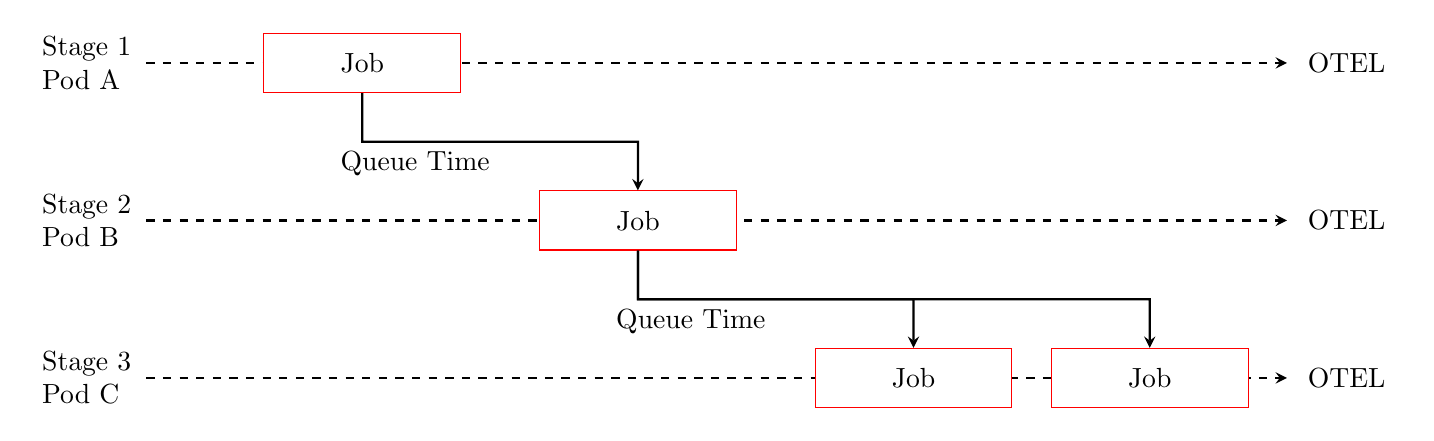
\begin{tikzpicture}[node distance=2cm]
        \pipelinetikz
        %%\draw [draw=red, thick] (2,0.5) rectangle (15,-4.5);
    \end{tikzpicture}}
    \raggedright

    \begin{description}
        \item[Freshness SLO]  X\% of results are processed in Y time or less over the last Z days.
        \item[Saturation SLO] X\% of results have Y queue time or less over the last Z days.
    \end{description}
    \note[item]{Jobs may take hours}
    \note[item]{Jobs may fan out or reduce}
    \note[item]{There is no root span}
\end{frame}

\begin{frame}
    \frametitle{Tracing Pipelines: How to FAIL}
    \centering
    \resizebox{\textwidth}{!}{%
    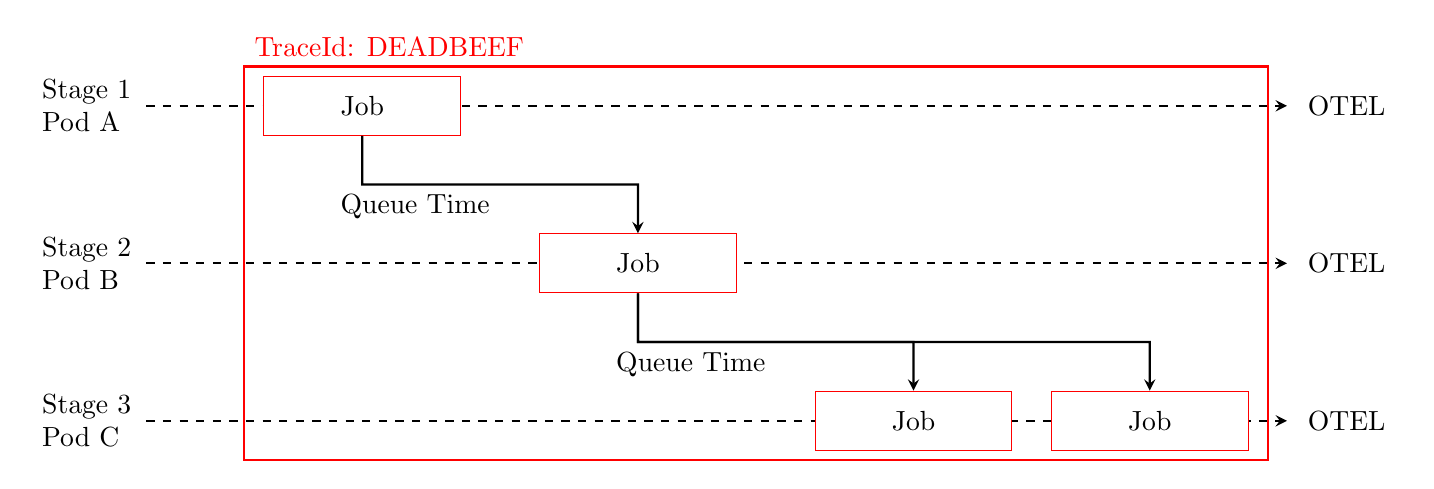
\begin{tikzpicture}[node distance=2cm]
        \pipelinetikz
        \draw [draw=red, thick] (2,0.5) node[anchor=south west, color=red] {TraceId: DEADBEEF} rectangle (15,-4.5);
    \end{tikzpicture}}
\end{frame}

\tikzstyle{process} = [
    rectangle,
    minimum width=2.5cm, 
    minimum height=0.75cm,
    text centered, 
    draw=red, 
    fill=white,
]
\begin{frame}
    \frametitle{Tracing Pipelines: Using Span Links}
    \centering
    \resizebox{\textwidth}{!}{%
    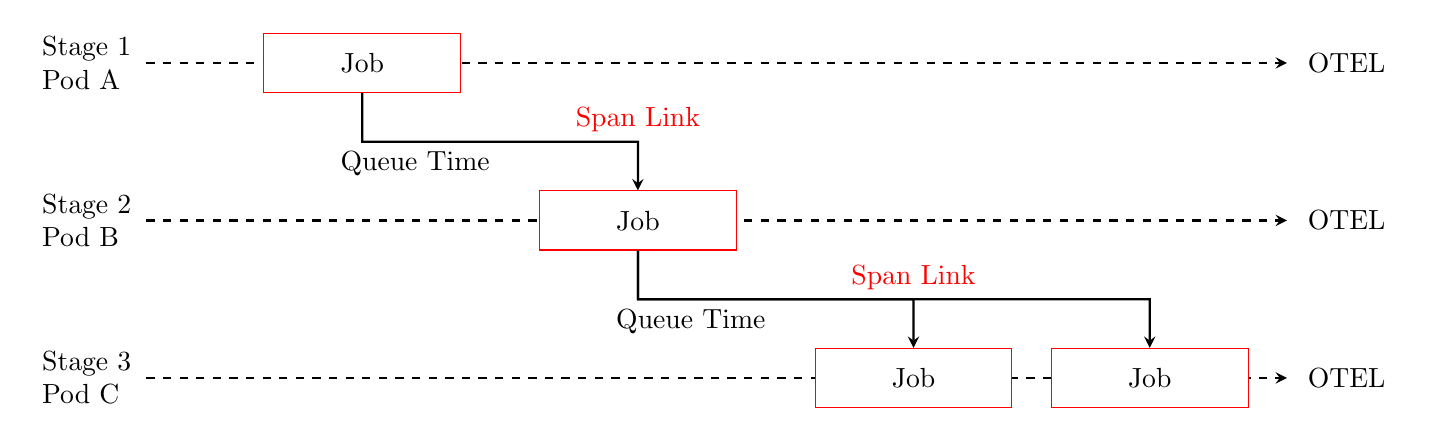
\begin{tikzpicture}[node distance=2cm]
        \pipelinetikz
        \node [color=red, anchor=south] at (7,-1) {Span Link};
        \node [color=red, anchor=south] at (10.5,-3) {Span Link};
    \end{tikzpicture}}
    \raggedright

    Create a TraceId per job and pass context across the bus.  Child jobs
    create a Span Link to reference the TraceId of the parent pipeline job.
\end{frame}

\begin{frame}[fragile]
    \frametitle{Tracing Pipelines: KISS Method}

    \begin{columns}
        \begin{column}{0.5\textwidth}
            Build a schema and pass meta information along the bus.
            \vskip 0.5cm
            Feedback loops for your teams.
        \end{column}
        \begin{column}{0.5\textwidth}
    \begin{figure}[h!]
        %%\begin{tabular}{c}
        \begin{lstlisting}[linewidth=4cm]
{
  custId        : int,
  discoveredTs  : Unix Epoch,

  stage1_traceId: string,
  stage1_status : int,
  stage1_startTs: Unix Epoch,
  stage1_stopTs : Unix Epoch,

  stage2_traceId: string,
  stage2_status : int,
  stage2_startTs: Unix Epoch,
  stage2_stopTs : Unix Epoch,

  stage3_traceId: string,
  stage3_status : int,
  stage3_startTs: Unix Epoch,
  stage3_stopTs : Unix Epoch
}
        \end{lstlisting}
        %%\end{tabular}
    \end{figure}
        \end{column}
    \end{columns}
\end{frame}
